\documentclass[12pt]{article}
\usepackage[a4paper,height=23cm]{geometry}
\usepackage[tableposition=top]{caption}
\captionsetup{font=small,labelfont=bf,labelsep=period,singlelinecheck=false,
  width=13cm}
\usepackage{color}
\usepackage{graphicx}
\usepackage{parskip}
\usepackage[hidelinks,linktoc=all,pdfpagemode=None]{hyperref}
\definecolor{darkblue}{rgb}{0.0,0.2,0.6}
\definecolor{darkgray}{rgb}{0.2,0.2,0.2}
\newcommand\blue[1]{\textcolor{darkblue}{#1}}
\newcommand\gray[1]{\textcolor{darkgray}{#1}}
\newcommand\I[1]{\rule{0pt}{#1}}
\newcommand\fishstat{{\sf fishstat}}
\newcommand\gt{\raisebox{0.1ex}\textgreater}
\newcommand\SOFIA{{\sf SOFIA}}
\newcommand\sofialink[2]{\blue{\href{https://github.com/sofia-taf/#1}{\sf #2}}}
\newcommand\sraplus{{\sf sraplus}}
\newcommand\TAF{{\sf TAF}}
\frenchspacing
\setlength{\tolerance}{300}
\setlength\hyphenpenalty{1000}
\hyphenation{calcu-lating reflect design develop-ment opposed experts control
  relevant report analysis}
\begin{document}

\thispagestyle{empty}

\begin{center}
  ~\\[0ex]
  \Large\bfseries Transparent Analytical Framework\\
  for Evaluating the Status of Stocks\\[1.5ex]
  \large{\rm SOFIA-TAF Design and Development Progress}\\[2.0cm]
  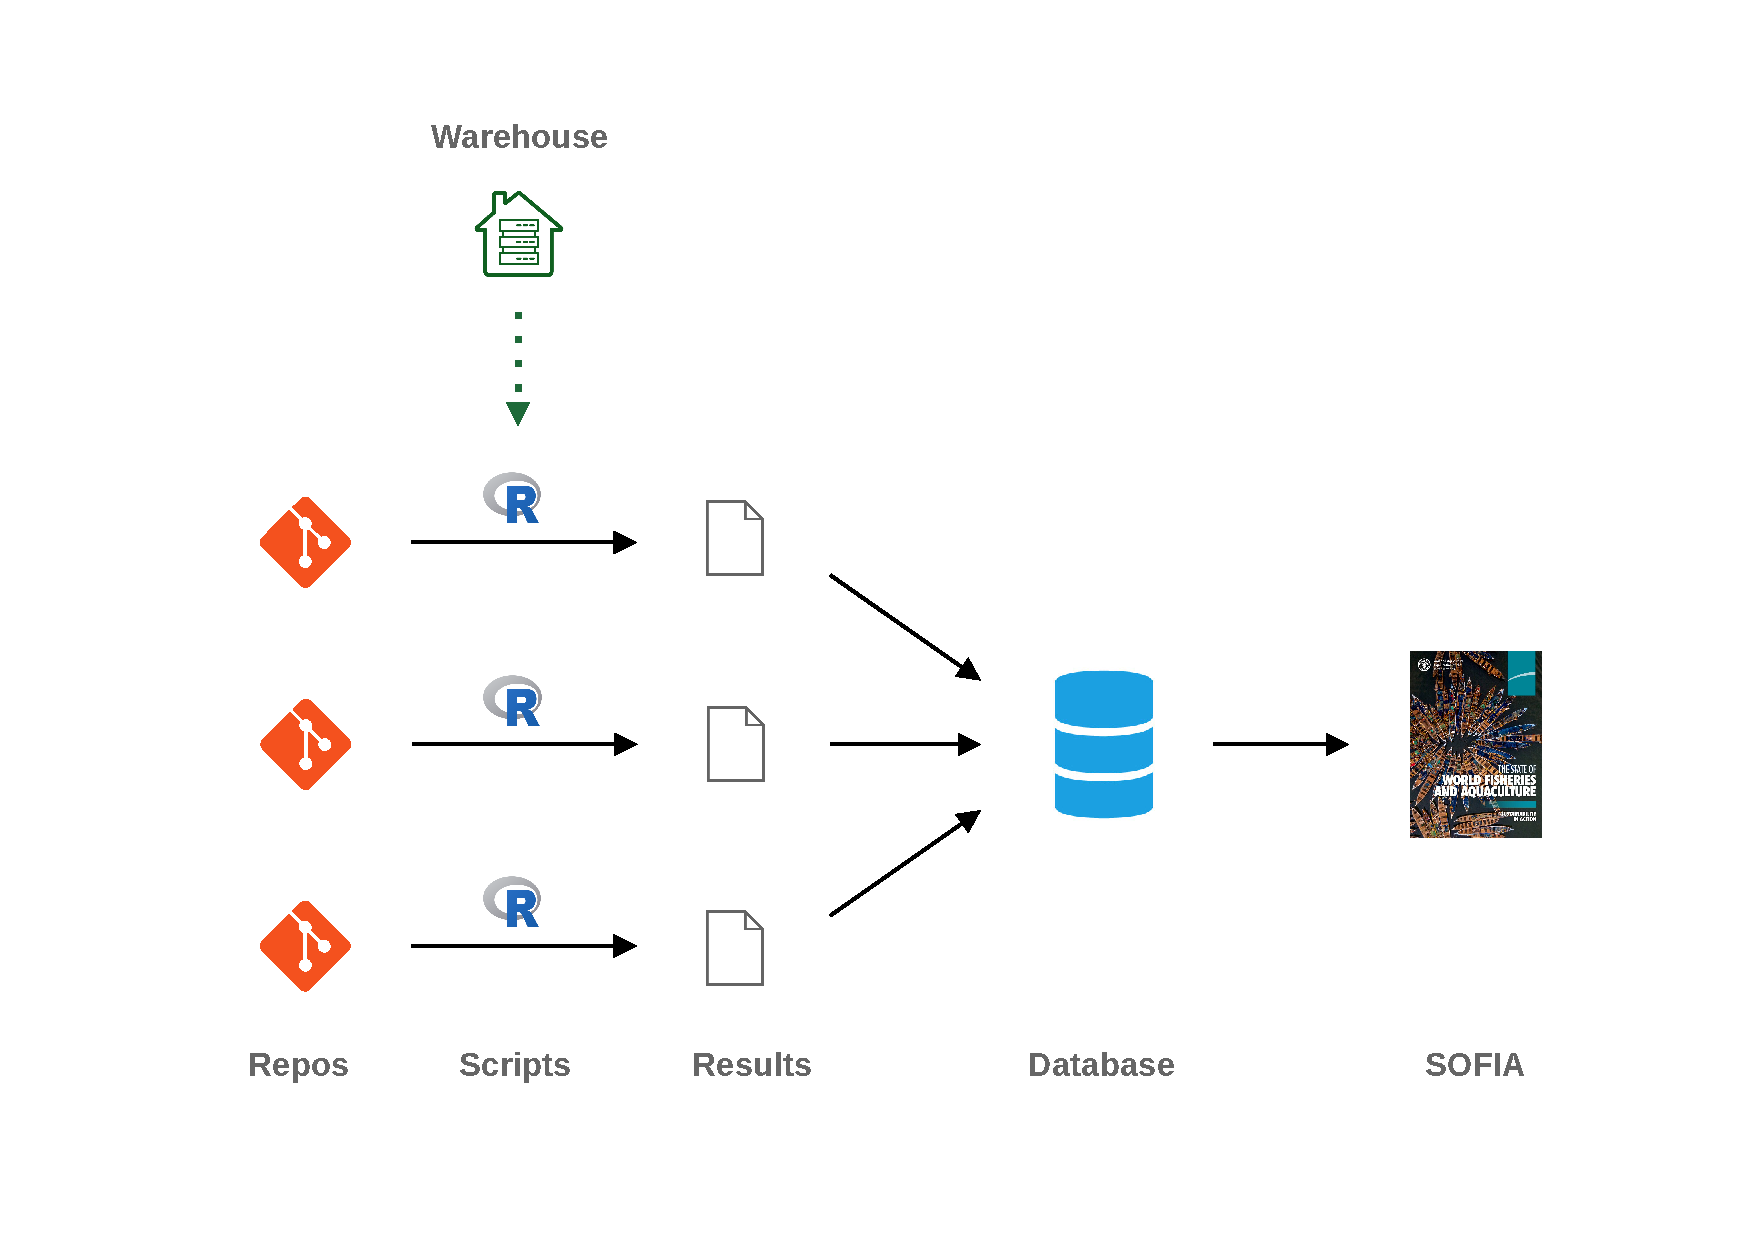
\includegraphics[width=0.64\textwidth]{sofia_taf_diagram}\\[1.5cm]
  \hspace{-1.5ex}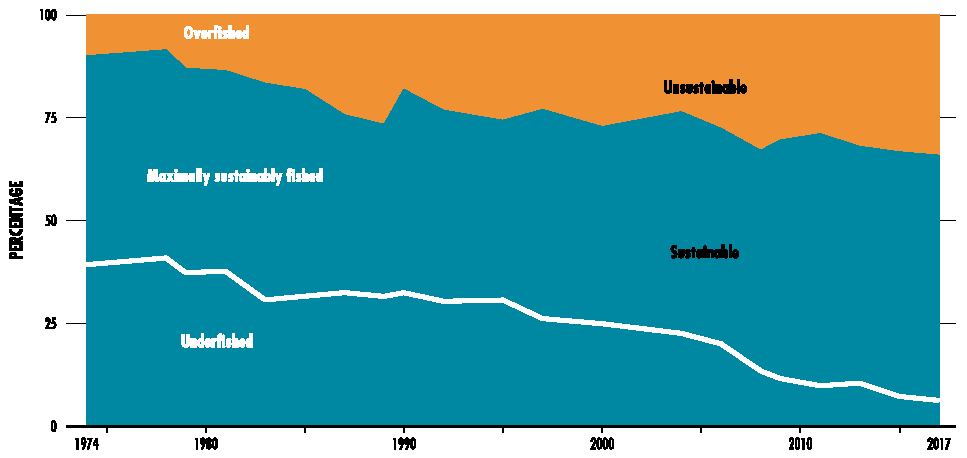
\includegraphics[width=0.75\textwidth]{sofia_fig19}\\[1.8cm]
  \mdseries Arni Magnusson\\[1.6ex]
  December 2024
\end{center}

\newpage

~\vspace{1em}
\setcounter{tocdepth}{2}
\tableofcontents

\newpage

\section{Executive summary}

This report gives a brief overview of the design and development progress of the
new SOFIA Transparent Analytical Framework (SOFIA-TAF) for evaluating the
status of stocks. The framework consists of four components:\\[-3ex]

\begin{itemize}
  \item SOFIA-TAF repositories, where each repository contains one analysis,\\
  calculating the status of stocks in a given area.\\[-3.5ex]
  \item Input data pathway, with fisheries data for all areas and
  stocks.\\[-3.5ex]
  \item SOFIA R package, a collection of utilities that are commonly used in\\
  SOFIA-TAF analyses.\\[-3.5ex]
  \item Database, storing the results from all SOFIA-TAF analyses.
\end{itemize}

This report uses a similar structure as the previous reports on SOFIA-TAF design
and development progress report (Magnusson 2021, 2022, 2023), updating each
section to reflect the current state of SOFIA-TAF. The main activities and
milestones achieved in 2024 are listed in Table \ref{tab:timeline-2024}.

\begin{table}[htb]\small
  \vspace{0.5ex}
  \caption{Overview of main activities and milestones in 2024.}
  \centering
  \begin{tabular}{rl}
    \hline
    Apr 2024 & Development update of the R package \fishstat\ to incorporate the
               newest\I{2.3ex}\\
    ~        & FAO FishStat data release.\\[0.8ex]
    ---      & Workshop with experts in Area 51 (W Indian Ocean).\\[0.8ex]
    May 2024 & Workshop with experts in 77 (E Pacific).\\[0.8ex]
    Oct 2024 & New version 2.1.3 of the R package \SOFIA\ released, with
               improved plots\\
    ~        & and a new color scheme.\\[0.8ex]
    ---      & Updated standard demos
               \sofialink{WorkshopEffortShared}{WorkshopEffortShared},
               \sofialink{WorkshopEffortByStock}%
               {WorkshopEffortByStock},\\[0.1ex]
    ~        & \sofialink{WorkshopIndexByStock}{WorkshopIndexByStock}, and
               \sofialink{WorkshopPriorsByStock}{WorkshopPriorsByStock} to use
               \SOFIA\ 2.1.3.\\[0.8ex]
    ---      & Workshop with experts in Area 61 (NW Pacific).\\[0.8ex]
    Dec 2024 & SOFIA-TAF repositories developed in 2024 are in Areas 51, 77, and
               87.\\[0.8ex]
    ---      & Progress report summarizes the overall design and the current\\
    ~        & development status.\\
    \hline
  \end{tabular}
  \label{tab:timeline-2024}
  \vspace{1ex}
\end{table}

At the end of this report is an appendix, listing Arni Magnusson's contributions
in 2024 to SOFIA-TAF design and development.

\newpage

% ______________________________________________________________________________

\section{Introduction}

\subsection{Background}

To provide a frame of reference behind the activities and milestones from
SOFIA-TAF development in 2024, it is worthwhile to quickly review the timeline
from 2021--2023 (Table \ref{tab:timeline-history}). See Magnusson (2021, 2022,
2023) for details.

\vspace{1ex}

\begin{table}[htb]\small
  \caption{Review of key activities and milestones in 2021--2023.}
  \centering
  \begin{tabular}{rl}
    \hline
    Mar 2021 & Initial design discussions.\I{2.3ex}\\[0.8ex]
    Nov 2021 & Initial development of the \SOFIA\ package.\\[0.8ex]
    Dec 2021 & Total of 12 SOFIA-TAF repositories on GitHub.\\[0.8ex]
    ---      & First design and development progress report.\\[0.8ex]
    Jan 2022 & \SOFIA\ package version 1.0 released.\\[0.8ex]
    May 2022 & First workshop with experts in Area 37 (Mediterranean and Black
               Sea).\\[0.8ex]
    Oct 2022 & SOFIA-TAF launch event at CAPAM Good Practices conference\\
    ~        & in Rome.\\[0.8ex]
    Dec 2022 & Total of SOFIA-TAF 32 repositories and 3 regional
               workshops.\\[0.8ex]
    Apr 2023 & Development of four standard demos that are used in regional
               workshops\\
    ~        & and in routine tests of the virtual research environment
               (VRE):\\[0.1ex]
    ~        & \sofialink{WorkshopEffortShared}{WorkshopEffortShared},
               \sofialink{WorkshopEffortByStock}%
               {WorkshopEffortByStock},\\[0.2ex]
    ~        & \sofialink{WorkshopIndexByStock}{WorkshopIndexByStock}, and
               \sofialink{WorkshopPriorsByStock}{WorkshopPriorsByStock}.
    \\[0.8ex]
    Jun 2023 & Initial development of R package \fishstat\ that provides FAO
               FishStat\\
    ~        & catch data in R format.\\[0.8ex]
    Dec 2023 & Total of 44 SOFIA-TAF repositories and 8 regional
               workshops.\\[0.8ex]
    \hline
  \end{tabular}
  \label{tab:timeline-history}
  \vspace{1ex}
\end{table}

\vspace{1ex}

Regional workshops (Table \ref{tab:workshops}) are of central importance for
introducing the new framework for evaluating the SOFIA status of stocks. The
workshops provide an opportunity to reach out to regional experts, demonstrate
the new analytical approach, and identify fisheries where additional data could
be submitted to FAO.

\vspace{1ex}

\begin{table}[htb]\small
  \caption{List of regional workshops.}
  \centering
  \begin{tabular}{clll}
    \hline
    Area & Short name        & Time     & Venue\I{2.3ex}\\
    \hline
    31   & W Atlantic        & 2022 Nov & Miami\I{2.3ex}\\
    34   & E Atlantic        & 2023 May & Banjul        \\
    37   & Med \& Black Sea  & 2022 May & Rome          \\
    41   & SW Atlantic       & 2022 Nov & Mar del Plata \\
    47   & SE Atlantic       & 2023 Dec & Cape Town     \\
    51   & W Indian Ocean    & 2023 Mar & Dar es Salaam \\
    ---  & W Indian Ocean II & 2024 Apr & Kochi         \\
    57   & E Indian Ocean    & 2023 Jan & Bangkok       \\
    61   & NW Pacific        & 2024 Oct & Rome          \\
    71   & W Pacific         & 2023 Nov & Bangkok       \\
    77   & E Pacific         & 2024 May & Mexico City   \\
    87   & SE Pacific        & 2024 Nov & Santa Marta   \\
    \hline
  \end{tabular}
  \label{tab:workshops}
  \vspace{1ex}
\end{table}

\newpage

\subsection{Objectives}

It is not for this author to define or prioritize the objectives of SOFIA-TAF to
support the overall analysis behind SOFIA. However, the following topics are
worth mentioning, as a context for some of the design decisions and features
that are being developed.\\[-1.5ex]

\begin{description}
  \item[Efficiency] is the ability to edit code in a single place to modify a
  large number of analyses, and to calculate top-level summary statistics from a
  large number of analyses.\\[-2.5ex]
  \item[Clarity] is the ability to easily navigate to a specific part of the
  analysis of a particular stock group and area, and to look up a specific
  result from one or more analyses.\\[-2.5ex]
  \item[Traceability] is the ability to backtrack exactly how a specific result
  was calculated, such as the status of a particular stock group in a given
  area.\\[-2.5ex]
  \item[Open science] is the ability to make the R scripts available online,
  along with the input data required for the scripts to run, inviting peer
  review of methodology and scientific collaboration.\\[-2.5ex]
  \item[Reproducibility] is the ability to run analyses on a variety of
  computers, e.g., a personal Windows laptop or a high-performance Linux
  cluster, to get the exact same result$\,$---$\,$also when the analysis is
  rerun months or years later.\\[-2.5ex]
  \item[Quality assurance] is the design and adoption of a workflow that reduces
  the probability of making human mistakes when preparing, modifying, running,
  and postprocessing the results from analyses.\\[-2.5ex]
  \item[Quality control] is the ability to identify where a human mistake has
  been made in a given analytical process, so the mistake can be located and
  corrected.\\[-1.5ex]
\end{description}

The initial development of SOFIA-TAF has focused especially on Tier 2 cases of
SOFIA analyses, where official stock assessments are not available, but catch,
effort, and survey index data exist as a basis for estimating stock status using
data-limited methods.

The SOFIA-TAF design also aims to serve as a platform to organize Tier 1
analyses (deriving stock status from official stock assessments) as well as
Tier~3 analyses (deriving stock status estimates from expert elicitation). These
tiers will require less R code than Tier 2 but use the same structure for R
scripts and data provenance to document exactly how the stock status was
calculated.

% ______________________________________________________________________________

\section{Design}

The SOFIA-TAF design (Figure \ref{fig:sofia-taf-diagram}) is based on
repositories containing R scripts that can read input data from files or
queries, to estimate the status of stocks. These results are then stored in a
database, which serves as the foundation for calculating summary statistics for
the final SOFIA report.

\begin{figure}[htb]
  \begin{center}
    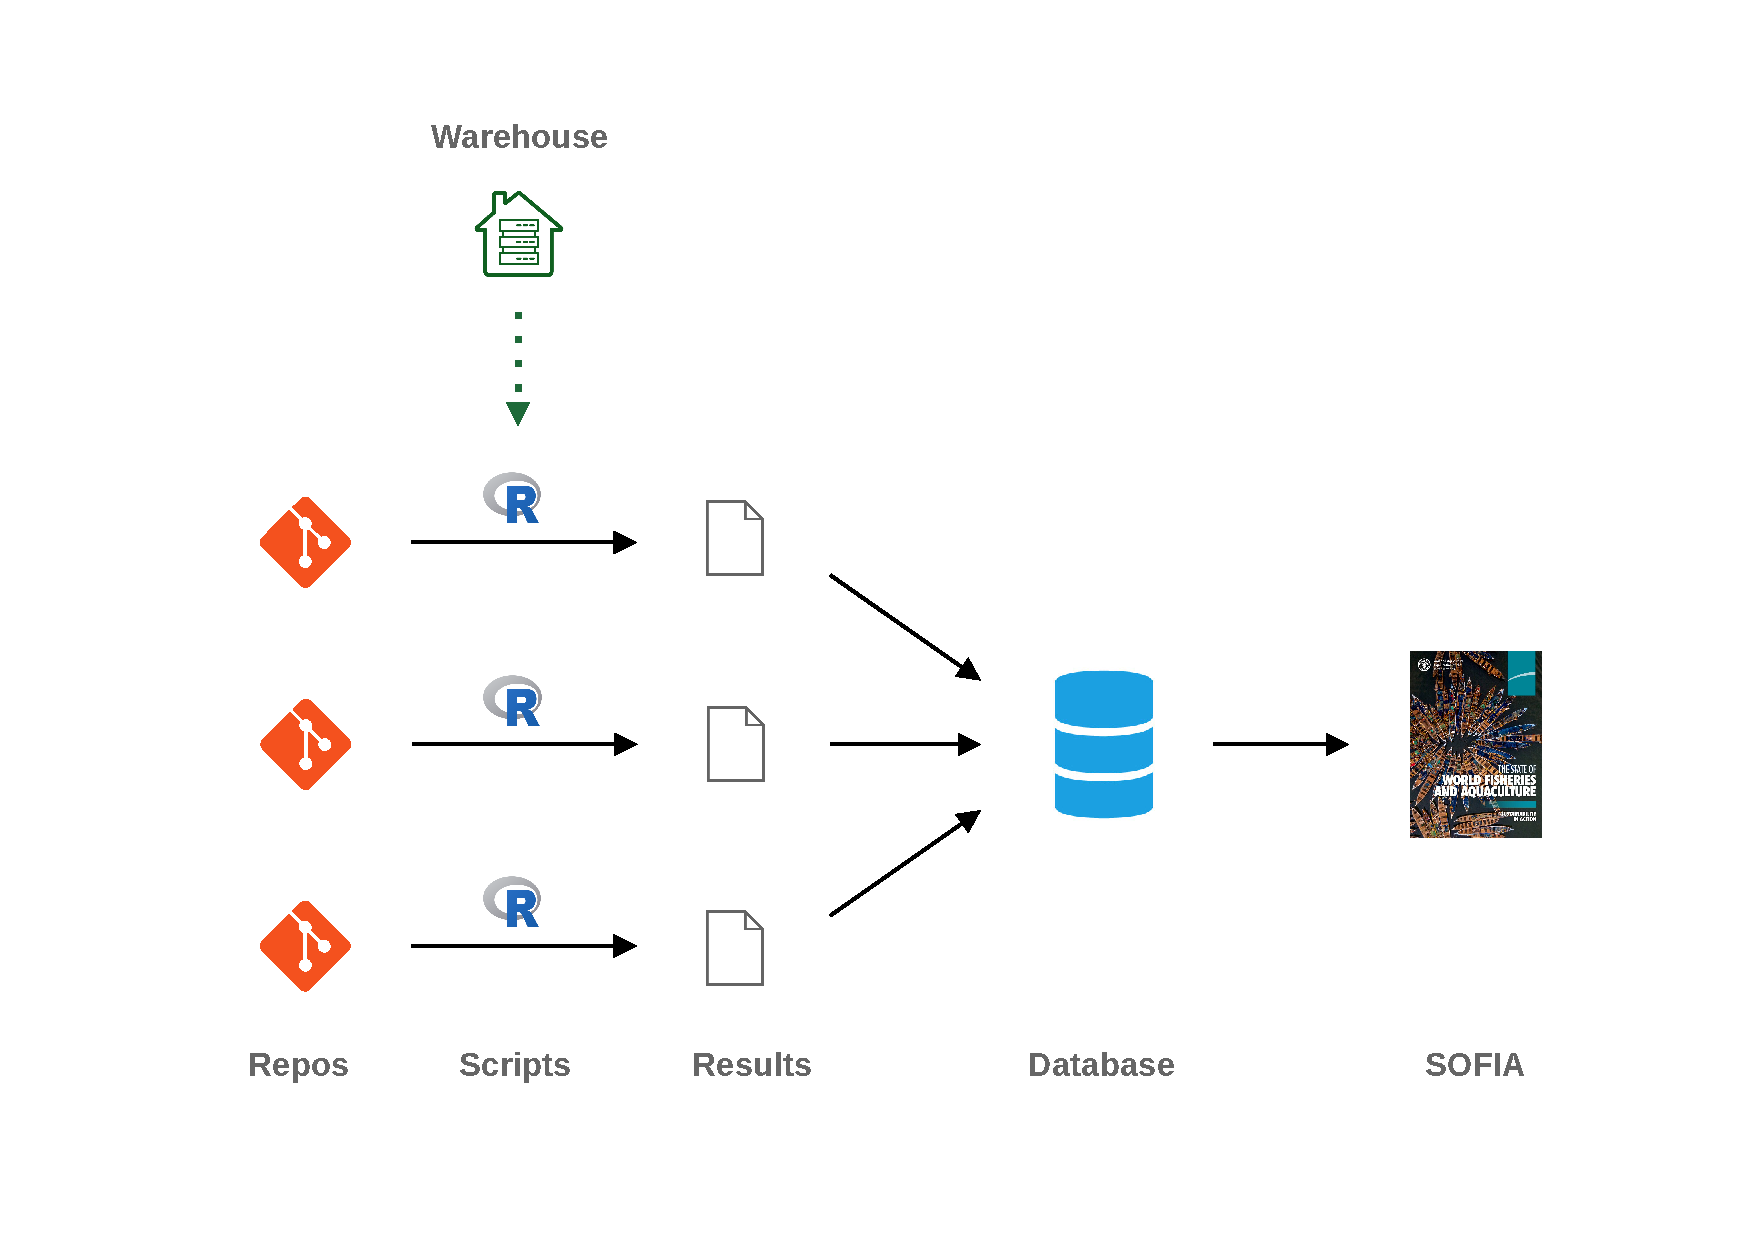
\includegraphics[width=0.8\textwidth]{sofia_taf_diagram}
    \vspace{2ex}
    \caption{SOFIA-TAF diagram, showing the flow of information from individual
      repositories (analyses of stocks and areas) to the final SOFIA report.}
    \label{fig:sofia-taf-diagram}
  \end{center}
\end{figure}

The scripts use a dedicated R package called \SOFIA. The next sections describe
each component of the SOFIA-TAF design in some detail: repositories, input data
pathway, \SOFIA\ R package, and the database.

\subsection{SOFIA-TAF repositories}

\subsubsection{Repository features}

Each SOFIA-TAF repository is a unit of analysis, corresponding to a specific
area and a set of stocks. A GitHub repository, sometimes abbreviated as `repo',
is an online directory that is especially convenient for organizing text files,
such as scripts and data files. GitHub repository features relevant for
SOFIA-TAF include:

\begin{itemize}
  \item Ability to make scripts available online, for browsing and downloading,
  along with the input data required for the scripts to run.
  \item Automatic backup of all files with the ability to return to previous
  saved states.
  \item Tracked changes showing who changed what and when, supporting online
  teamwork.
  \item Ability to tag specific saved states of the analysis and give them
  descriptive names, such as `starting point`, `2021 data` or `results imported
  to database`.
  \item Ability to upload large attachments (\gt 100 MB) to accompany tagged
  states.
  \item Online facilities to compare text files and view changes, line by line.
\end{itemize}

\subsubsection{R scripts}

The analysis inside each repository consists of a set of R scripts that are
organized in TAF format (Magnusson and Millar 2023). This means there are four
standard scripts
(Table~\ref{tab:taf-scripts}) that conduct and document the analysis:\\[-1ex]

\begin{table}[htb]\small
  \caption{Standard TAF scripts for a given analysis.}
  \centering
  \begin{tabular}{ll}
    \hline
    Script          & Purpose\I{2.4ex}                                 \\
    \hline
    \verb|data.R|   & Preprocess data, write TAF data tables\I{2.5ex}  \\[0.4ex]
    \verb|model.R|  & Run analysis, write model results                \\[0.4ex]
    \verb|output.R| & Extract
                      results of interest, write TAF output tables     \\[0.4ex]
    \verb|report.R| & Prepare plots and formatted tables               \\[0.3ex]
    \hline
  \end{tabular}
  \label{tab:taf-scripts}
  \vspace{1.5ex}
\end{table}

The TAF scripts are run sequentially, each reading files that were created in a
previous step. The first script, \verb|data.R|, reads data files that were
declared and documented in a \verb|DATA.bib| text file. A similar
\verb|SOFTWARE.bib| file can be used to declare specific versions of software
used in the analysis, to strengthen reproducibility.

\begin{figure}[htb]
  \begin{center}
    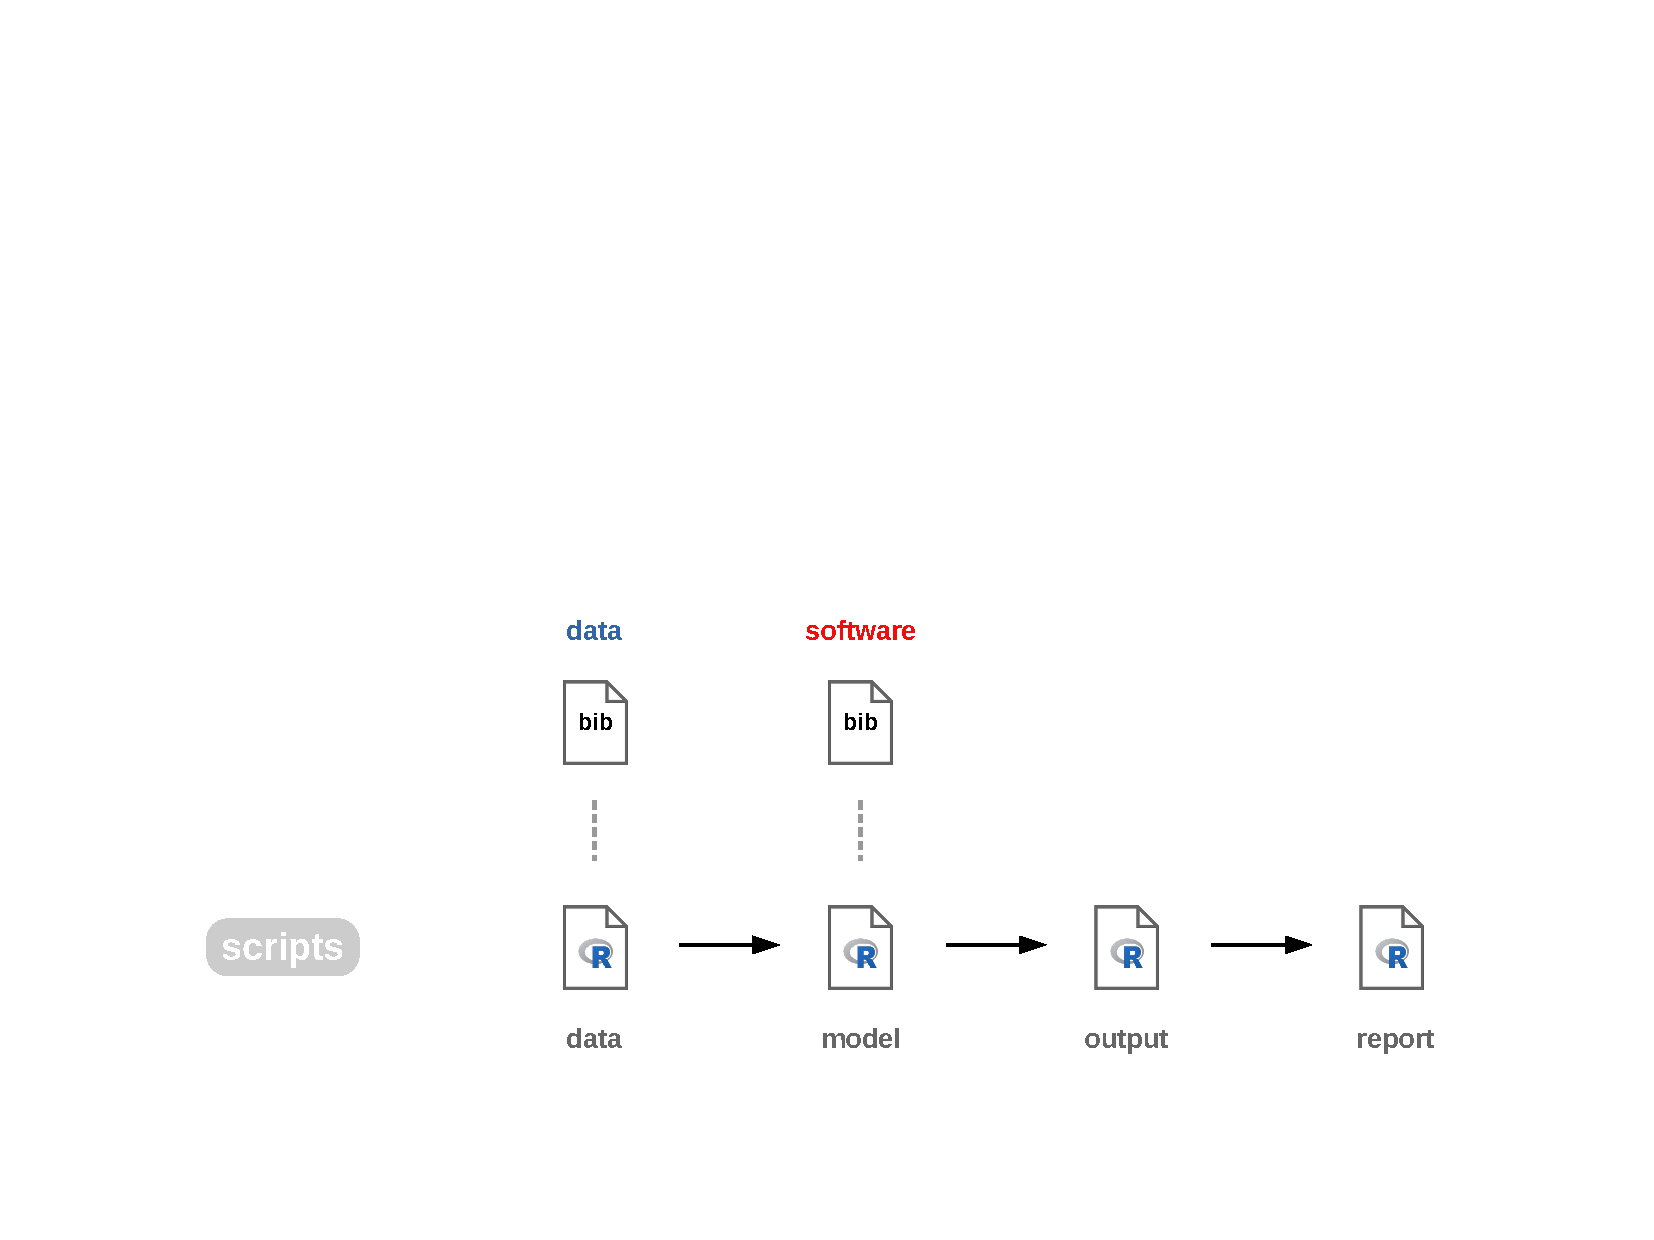
\includegraphics[width=0.8\textwidth]{taf_diagram}
    \vspace{2ex}
    \caption{TAF scripted workflow. Each SOFIA-TAF repository/analysis contains
      four standard R~scripts that are run sequentially. The initial data and
      software are declared in so-called bib files.}
    \label{fig:taf-diagram}
  \end{center}
\end{figure}

\newpage

The R scripts conducting SOFIA-TAF analyses rely especially on three R
packages:\\[-2ex]

\begin{itemize}
  \item \SOFIA\ -- a dedicated package to support SOFIA-TAF\\
  (Sharma and Magnusson 2024)
  \item {\sf TAF} -- utilities to manage scripts, data files, metadata, and R
  data objects\\
  (Magnusson and Millar 2023)
  \item \sraplus\ -- biomass dynamics model with Bayesian priors\\
  (Ovando 2022)
\end{itemize}

\subsubsection{Repository names and directory structure}

GitHub repositories are given descriptive names, such as

\qquad\blue{\url{https://github.com/sofia-taf/2021Area37Coastal}}

for the analysis started in 2021 of coastal stocks in Area 37.

On a personal laptop or a high-performance cluster, the SOFIA-TAF repositories
are organized in a hierarchical directory structure (Figure
\ref{fig:sofia-taf-dirs}), similar to the repository name as year/area/stock
group.\\

\begin{figure}[htb]
  \begin{center}
    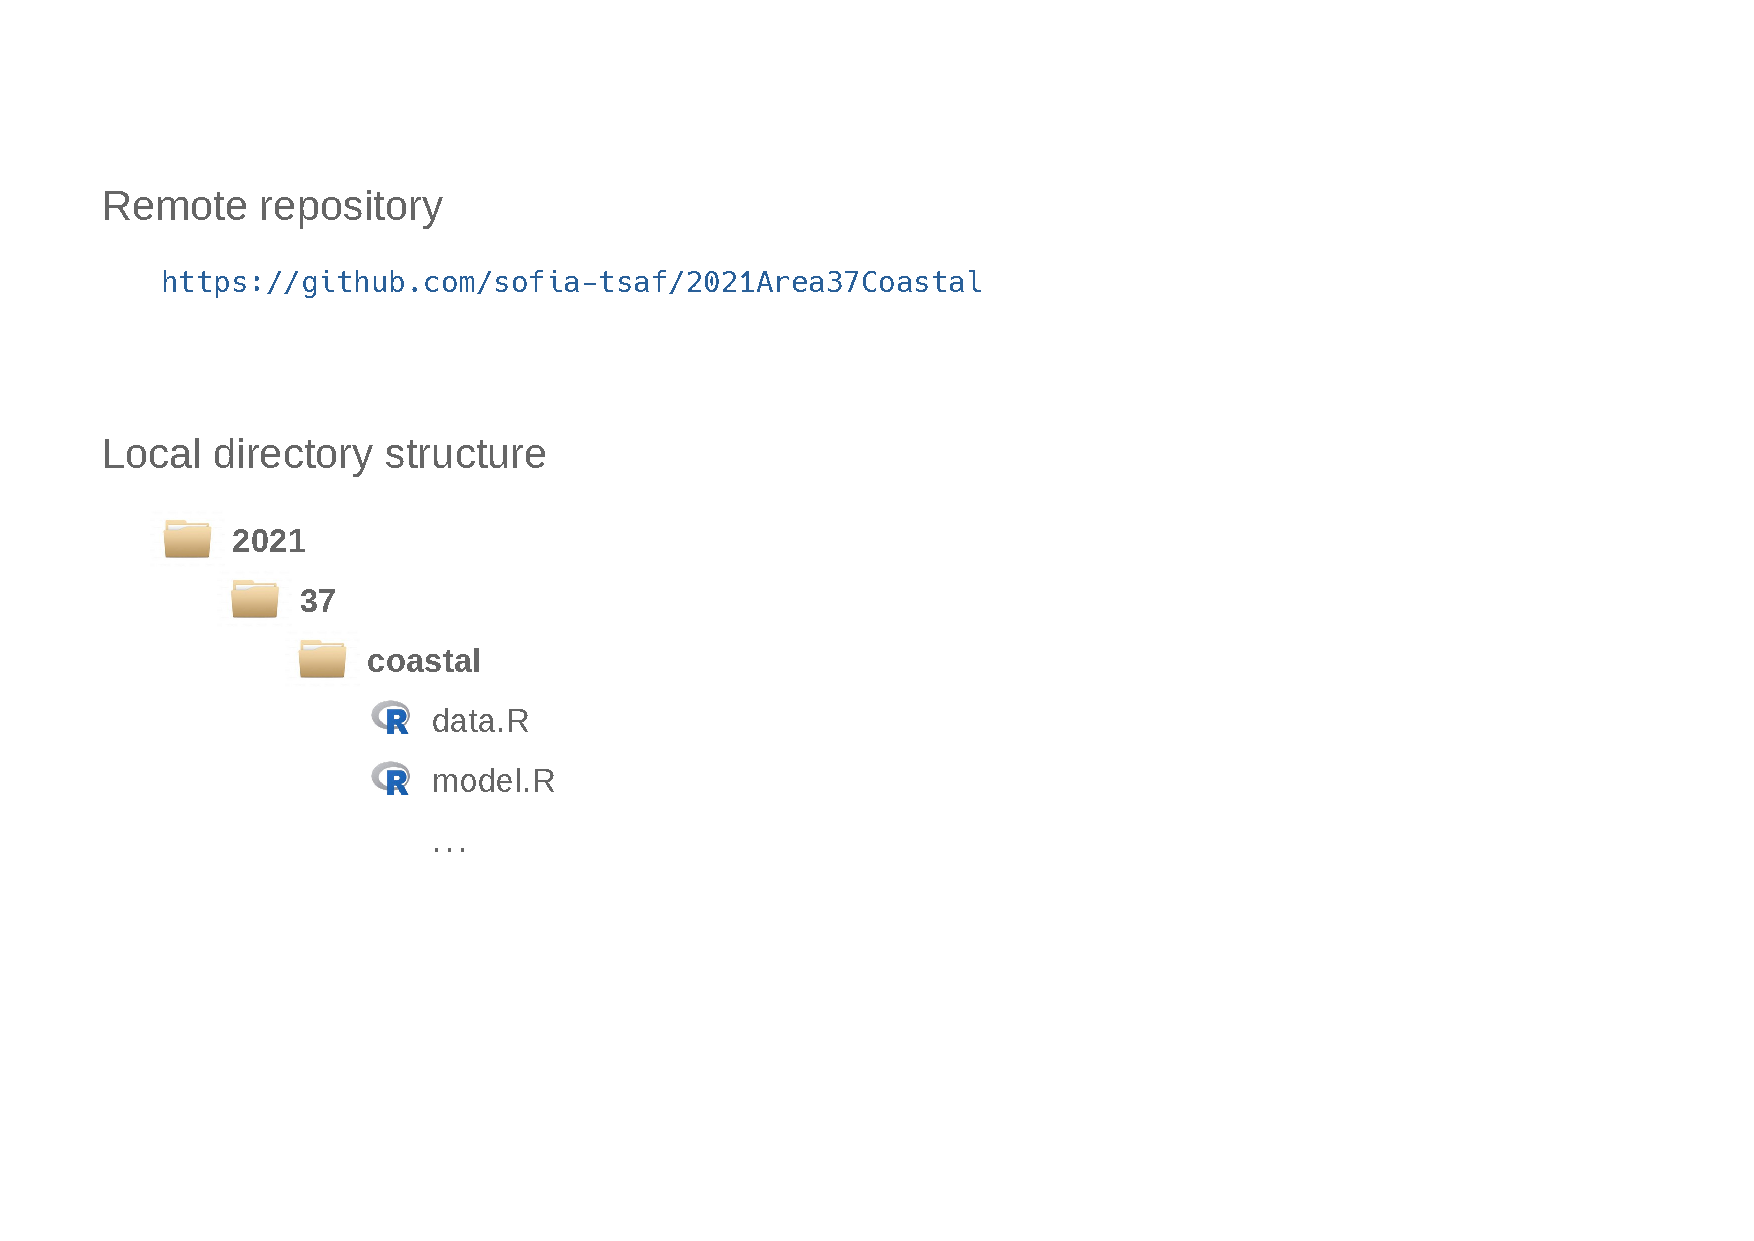
\includegraphics[width=0.6\textwidth]{sofia_taf_dirs}
    \vspace{1ex}
    \caption{SOFIA-TAF local directory structure, showing the similarity between
      the remote repository name and the local directory names.}
    \label{fig:sofia-taf-dirs}
  \end{center}
\end{figure}

\vspace{1ex}

This hierarchical directory structure is practical to navigate and run the
analyses, access results, and run top-level summary calculations across a large
number of analyses.

\newpage

\subsection{Input data pathway}

\subsubsection{Data collection templates}

SOFIA-TAF input data are collected and prepared in a collaborative process
between FAO and regional experts. The data used within a Tier 2 analysis are
organized in files such as \verb|catch.csv|, \verb|effort.csv|, and
\verb|index.csv|, containing multiple stocks in each file. Data provided by
regional experts, however, are termed {\it primary} data files and are organized
as one file per stock, using filenames such as
\verb|Yellowtail_snapper_Mexico.csv|. The conversion from primary data files to
Tier 2 input data files is handled by the \SOFIA\ package.

\subsubsection{The fishstat R package}

As of December 2024, all SOFIA-TAF analyses start with catch data uploaded as
a \verb|catch.csv| text file in CSV format.

An alternative input data pathway could be used for the catch data by reading
directly from the FAO FishStat database. To facilitate this pathway, development
was started in 2023 to create an R package called \fishstat\ that provides
FishStat catch data in R format as data frames.

Reading catch data directly from FishStat, rather than uploading handcrafted
text files, would be an improvement and result in a more streamlined workflow
that is traceable and quality-controlled.

The development of the \fishstat\ R package will be continued in 2025.

\subsubsection{Input data warehouse}
\label{subsubsec:design-data-warehouse}

Dedicated GitHub repositories can be used to host data that are used across many
analyses:

\begin{itemize}
  \item \blue{\url{https://github.com/sofia-taf/catches}} for catch data
  collections other than FishStat.
  \item \blue{\url{https://github.com/sofia-taf/effort}} for effort data by year
  and area.
\end{itemize}

These repositories offer a central place for SOFIA-TAF input data where they can
be updated, documented, and quality checked.

\subsection{SOFIA R package}

The \SOFIA\ package (Sharma and Magnusson 2024) contains utilities that are
commonly used in SOFIA-TAF analyses. It is developed in a dedicated GitHub
repository:

\qquad\blue{\url{https://github.com/sofia-taf/SOFIA}}

The \SOFIA\ package provides a single place to modify a large number of
SOFIA-TAF analyses. Incremental improvements become more manageable, e.g.,
changing the format of a specific plot, without having to edit each and every
SOFIA-TAF analysis. It also makes the R scripts for each analysis shorter and
thus easier to read, write, and maintain.

\subsection{Database}

The database will contain the results from all the individual SOFIA-TAF
analyses. The results describe the status of stocks by FAO Major Fishing Areas,
both in numerical terms and in categorical terms: underfished, fully fished, and
overfished.

The only way to enter stock status results into the database is via SOFIA-TAF
analyses, as indicated in the design diagram (Figure
\ref{fig:sofia-taf-diagram}), and when analyses of a specific areas and stocks
are updated, the database is automatically updated. Furthermore, the top-level
analysis for the final SOFIA report, aggregating a large number of SOFIA-TAF
analyses, should be based on queries to the database.

The above design guarantees the traceability of SOFIA results, all the way from
the individual datasets and analyses to the final published report.

The database is also a convenient stage in the pipeline to apply quality
control. Examples of quality checks could include referential integrity of
species and stock names, summary statistics at different levels of aggregation,
counting stocks in each area, plotting the distribution of numerical stock
status, etc. This will ensure that all stocks are accounted for, and reveal any
inconsistencies or issues that should be checked in the underlying analyses.

\newpage

% ______________________________________________________________________________

\section{Development status and next steps}

\subsection{SOFIA-TAF repositories}

\subsubsection{Current status}

As of end of December 2024, the GitHub site
\blue{\url{https://github.com/sofia-taf}} contains 49 SOFIA-TAF repositories, 12
that were created in 2021, 20 were created in 2022, 12 were created in 2023, and
5 were created in 2024 (Table \ref{tab:repository-count}).

\begin{table}[htb]\small
  \caption{Overview of SOFIA-TAF repositories.}
  \centering
  \begin{tabular}{llrl}
    \hline
    ~ & ~ & Number of\I{2.4ex}\\
    Year & Area & analyses & Specifically\\
    \hline
    2021 & Area 31   &  1 & Test\I{2.4ex}\\[0.2ex]
    ~    & Area 37   & 11 & ClamsOK, Coastal, Cods, Demersal, Flounder,\\
    ~    & ~         &  ~ & Herring, Other, Shads, Shimps, Squid, Test\\[0.5ex]
    2022 & Area 31   & 10 & CatchEffortGlobalv2JM, CatchOnly,\\
    ~    & ~         &  ~ & DemoEffortByStock, DemoEffortShared,\\
    ~    & ~         &  ~ & DemoIndexByStock, EffortJMstcks,\\
    ~    & ~         &  ~ & effortlocalcatchlocalv2JM, IndexMethodv2JM,\\
    ~    & ~         &  ~ & Indexstocks, Testnewstocks\\[0.2ex]
    ~    & Area 37   &  2 & Clams, Demo\\[0.2ex]
    ~    & Area 41   &  3 & DemoPriorsByStock, RelevantStocks\\[0.2ex]
    ~    & Area 57   &  4 & Efforttest, EffortTestNoPriornew70yrstocks,\\
    ~    & ~         &  ~ & Tier2FAOMonitored31withdepPrior,\\
    ~    & ~         &  ~ & Tier2FAOMonitorednodepPrior\\[0.2ex]
    ~    & Deep Seas &  1 & CCAMLR\\[0.5ex]
    2023 & Area 34   &  4 & Decapterus, DemersalsSouthLocalEffort,\\
    ~    & ~         &  ~ & GlobalEffortFishstatstocks, Loligo\\[0.2ex]
    ~    & Area 51   &  2 & Demo, ShortDemo\\[0.2ex]
    ~    & Area 57   &  5 & 33MonitoresStockssraplusSathia, Demo,\\
    ~    & ~         &  ~ & FAOnonmonitoredstcks70yrs,\\
    ~    & ~         &  ~ & NonMonStocks-25-50yrs, NonMonStocks50-69yrs\\[0.2ex]
    ~    & Area 71   &  1 & FishStat30\\[0.5ex]
    2024 & Area 51   &  1 & Fishstat\\[0.2ex]
    ~    & Area 77   &  3 & Fishstat, Tier2Manual, Tier2FishstatJ\\[0.2ex]
    ~    & Area 87   &  1 & Tier2\\[0.1ex]
    \hline
  \end{tabular}
  \label{tab:repository-count}
  \vspace{1.5ex}
\end{table}

The status of all of these analyses is exploratory for development purposes, as
opposed to production analyses for a final SOFIA report. Each SOFIA-TAF analysis
declares the version of the \SOFIA\ package used, so the analysis can be rerun
at a later point and produce consistent results.

In addition to the main GitHub site \blue{\url{https://github.com/sofia-taf}},
another site \blue{\url{https://github.com/sofia-taf-dev}} has been created, as
an alternative place to organize development. One approach to manage SOFIA-TAF
would be store experimental analyses on the `dev' site and production analyses
on the main site.

Four demo repositories are used in regional workshops and in routine tests of
the virtual research environment (VRE):

\begin{itemize}
  \item \sofialink{WorkshopEffortShared}{WorkshopEffortShared}
  \item \sofialink{WorkshopEffortByStock}{WorkshopEffortByStock}
  \item \sofialink{WorkshopIndexByStock}{WorkshopIndexByStock}
  \item \sofialink{WorkshopPriorsByStock}{WorkshopPriorsByStock}
\end{itemize}

These four demos serve as a reference for SOFIA-TAF, demonstrating standardized
scripts for analyzing various combinations of effort data, survey index data,
and priors. As reference analyses, they will be updated and synchronized when
changes and improvements are introduced in the \SOFIA\ package and other
components of the SOFIA-TAF framework.

\subsubsection{Next steps}
\label{subsubsec:repos-next-steps}

\textbf{Read catch data from the fishstat package}

The current development state of the \fishstat\ R package is ready for testing.
A test repository would start from an existing analysis and then replace the
\verb|catch.csv| file with an R script that extracts the catch data from the
\fishstat\ package. If the \verb|catch.csv| file contained catch data from the
FishStat database, then the two input pathways should produce the same input
data. The \fishstat\ package offers a more efficient, traceable, and
quality-controlled workflow.\\[-2ex]

\textbf{Tier 1 and 3}

All the current SOFIA-TAF repositories developed so far correspond to Tier 2
analysis. Tests of Tier 1 and/or Tier 3 analyses are likely to be scheduled in
2025, involving numerical and categorical data from official stock assessments
and expert elicitation. This will further increase the clarity and traceability
of the overall SOFIA analysis of stock status.\\[-2ex]

\textbf{Managing repositories}

During the development of SOFIA-TAF, a number of experimental analyses have been
created as repositories on the main \blue{\url{https://github.com/sofia-taf}}
site. Some analyses are likely to become production analyses for a final SOFIA
report, whose results should be imported into the database of SOFIA-TAF results,
while other analyses could be put aside and migrated to the development area
on\linebreak \mbox{\blue{\url{https://github.com/sofia-taf-dev}}}. Some older
experimental analyses could be deleted, if they have been superseded by more
recent analyses.\\[-2ex]

When importing results from analyses into the database of SOFIA-TAF results, the
relevant analyses could be defined as all repositories on
\blue{\url{https://github.com/sofia-taf}} whose name begins with year and area.

\textbf{Managing output files}

A significant challenge in SOFIA-TAF is that each analysis takes considerable
time to run (\gt 1 hr) and produces large output files (\gt 100 MB). Every time
a small update is made to the scripts or underlying data, a new run is required
and the output files are likely to change. SOFIA-TAF development so far has
explored two approaches to store the output files.

Approach 1. Initial development (e.g., \verb|area37|) kept the output files
outside of the repository. Instead of uploading the output files along with the
R scripts, output files were uploaded as GitHub `release assets'. The advantage
of this approach is that the repository remains very light and easy to work
with, and takes much less space on the hard drive of a personal laptop.

Approach 2. Later development (e.g., \verb|2021Area37Coastal|) has the output
files stored inside the repository. The advantage of this approach is that it
reduces the need to manage tags and GitHub releases, and makes it slightly less
likely to have mismatching R scripts and output files.

Unfortunately, neither of the above approaches can guarantee a correct match
between the R scripts and the output files. In other words, when a change is
made to an R script and uploaded to the repository, it's easy to forget or omit
running the entire analysis and uploading new output files.

A 3rd approach worth exploring would be not to upload output files to the GitHub
repository at all. Instead, the database server would run all analyses locally.
Specifically, a GitHub webhook could be developed, so that whenever a change is
uploaded to the GitHub repository, the database server pulls the changes, runs
the analysis and imports the results into the database. This would guarantee a
strong linkage between the SOFIA-TAF repositories and the database.

\subsection{Input data pathway}

\subsubsection{Current status}

The \fishstat\ R package is being developed in a public repository,
\blue{\url{https://github.com/sofia-taf/fishstat}}. It is now ready for testing
(see Section \ref{subsubsec:repos-next-steps}: Read catch data from the
\fishstat\ package).

The input data warehouse \blue{\url{https://github.com/sofia-taf/catches}}
repository currently contains one file \verb|cap_2021-10-17_193245.csv| with
catch data. The \blue{\url{https://github.com/sofia-taf/effort}} repository has
been created but is still empty.

\newpage

\subsubsection{Next steps}

Once testing has completed, the \fishstat\ R package will be announced, possibly
with a short journal communication.

Effort data by year and area can be added to the \verb|effort| repository in CSV
format. These general effort series are used when stock-specific effort data are
not available.

\subsection{SOFIA R package}

\subsubsection{Current status}

Version 2.1.3 of the \SOFIA\ package was released on 8 October 2024. The package
help page that comes with \SOFIA\ lists the following functions, categorized by
functionality.\\[-2ex]

{\it Prepare data:}

\begin{tabular}{ll}
  \verb|addDriors|   & add driors column to stocks object\\
  \verb|addEffort|   & add effort column to catch data\\
  \verb|addIndex|    & add index column to catch data\\
  \verb|convertData| & convert primary data to combined data\\
  \verb|groupData|   & group primary data in subdirectories\\[1.5ex]
\end{tabular}

{\it Calculate:}

\begin{tabular}{ll}
  \verb|calcCat| & stock status categories\\[1.5ex]
\end{tabular}

{\it Plot:}

\begin{tabular}{ll}
  \verb|plotCat| & summary of stock status categories\\[1.5ex]
\end{tabular}

{\it Repositories:}

\begin{tabular}{ll}
  \verb|gitRepos|    & list GitHub repositories\\
  \verb|gitClone|    & clone GitHub repository\\
  \verb|gitCloneAll| & clone all SOFIA-TAF repositories\\[1.5ex]
\end{tabular}

The current status of the package is stable and fully documented, passing a
strict \verb|R CMD --as-cran| quality check. Table \ref{tab:package-history}
shows the complete release history.

\newpage

\begin{table}[htb]\small
  \caption{\SOFIA\ package release history.}
  \centering
  \begin{tabular}{lrl}
    \hline
    Version & Date & New functions\\
    \hline
    2.1.3   & 2024-10-08 & ~\I{2.3ex}\\
    2.1.2   & 2023-05-19 & ~\\
    2.1.1   & 2022-11-15 & ~\\
    2.1.0   & 2022-11-11 & \verb|addIndex|\\[0.5ex]
    2.0.0   & 2022-08-08 & \verb|gitRepos|, \verb|gitClone|,
                           \verb|gitCloneAll|\\[0.5ex]
    1.2.1   & 2022-05-21 & ~\\
    1.2.0   & 2022-02-25 & \verb|convertData|\\[0.5ex]
    1.1.0   & 2022-02-20 & \verb|groupData|\\[0.5ex]
    1.0.3   & 2022-02-14 & ~\\
    1.0.2   & 2022-01-24 & \verb|addDriors|, \verb|addEffort|, \verb|calcCat|,
                           \verb|plotCat|\\
    \hline
  \end{tabular}
  \label{tab:package-history}
  \vspace{1.5ex}
\end{table}

A more detailed list of changes introduced in each version of the \SOFIA\
package can be found online at
\blue{\url{https://github.com/sofia-taf/SOFIA/blob/main/NEWS.md}}.

\subsubsection{Next steps}

\textbf{Prior on carrying capacity}

With the accumulated experience of applying the \sraplus\ model to a wide
variety of stocks, it seems that in some cases it might be helpful to use a
prior distribution on carrying capacity $K$. This could keep the estimated value
of $K$ within a realistic range. The \SOFIA\ package could assist the user in
setting a reasonable prior on $K$, based on the historical catches, specifically
the \verb|format_driors| arguments \verb|k_prior| and \verb|k_prior_cv|. Such a
prior could either be applied by default for all stocks or enabled for specific
stocks as necessary.\\[-2ex]

\textbf{Generalized prior input file}

Currently, the prior input file is parsed expecting certain content to be found
in the \verb|priors.csv| file, specifically the columns \verb|initial_state|,
\verb|initial_state_cv|, \verb|terminal_state|, and \verb|terminal_state_cv|. An
improved interface would allow the user to specify any priors, including
\verb|k_prior| and \verb|growth_rate_prior|.\\[-2ex]

\textbf{New plots}

New plots could be implemented, inspired by the JARA package (Winker et al.
2020), showing $B/B_\mathrm{MSY}$ and $F/F_\mathrm{MSY}$ time series as dots,
median, and confidence regions.\\[-2ex]

\newpage

\textbf{Fixed random seed}

When many workshop participants run the same example, they seem to get slightly
different results. This could be caused by different random seeds used in the
Markov chain Monte Carlo (MCMC) analysis. However, the sraplus function
\verb|fit_sraplus| has a default \verb|seed = 42| that all workshop participants
were probably using. It would be worth looking into how the random seed is
handled by the \sraplus\ package, as using a fixed random seed would strengthen
the reproducibility of SOFIA-TAF analyses.\\[-2ex]

\textbf{Quality control}

One area of the \SOFIA\ package that can be developed is the creation of quality
control functions for SOFIA-TAF analyses, identifying possible mistakes in the
analyses that can then be fixed.

\subsection{Database}

\subsubsection{Current status}

A new database has been developed by FAO to store SOFIA-TAF results. The
presentation by Anton Ellenbroek at regional workshops from 2023 onward gives an
outline of the objectives, design, and functionality of this database.

\subsubsection{Next steps}

\textbf{Strong link between repositories and database}

The link between SOFIA-TAF repositories and the database of results (Figure
\ref{fig:sofia-taf-diagram}) is essential for traceability and the fundamental
purpose of SOFIA-TAF. The very basis of the SOFIA-TAF design is that the results
found in the database should match exactly the results produced by the SOFIA-TAF
repositories.

The design and development of this linkage is still ongoing, including automatic
detection of which analyses contain results that should be imported into the
database. The separation of repositories into production analyses on
\blue{\href{https://github.com/sofia-taf}{\sf sofia-taf}} and experimental
analyses on \blue{\href{https://github.com/sofia-taf-dev}{\sf sofia-taf-dev}}
(Section \ref{subsubsec:repos-next-steps} on `Managing repositories') is related
to designing a strong link between repositories and the database of SOFIA-TAF
results.

\textbf{Database server managing SOFIA-TAF output files}

One design possibility is to have a dedicated SOFIA-TAF database server as the
main platform to run SOFIA-TAF analyses and manage output files, in addition to
importing the results into the database.

The development goal `Managing output files' (Section
\ref{subsubsec:repos-next-steps}) elaborates on this possible approach, which
could involve a GitHub webhook to establish a reliable pipeline of information
from SOFIA-TAF repositories to the database.

\vspace{3ex}

% ______________________________________________________________________________

\section{Acknowledgements}

Working with Rishi Sharma on this project is a privilege and joy. Our domains of
expertise complement each other, and we share a common vision and enthusiasm to
enhance the FAO infrastructure and analytical workflows for estimating the state
of the world's fisheries. I would like to acknowledge Colin Millar for our
collaboration in creating TAF (Magnusson and Millar 2023), which has served as
an inspiration and basis for the SOFIA-TAF design. I thank Anton Ellenbroek for
leading the development of a database storing SOFIA-TAF results. Last but not
least, I am grateful to Pedro Barros and colleagues at FAO for their guidance
and vote of confidence for this technical development project.

\vspace{3ex}

% ______________________________________________________________________________

\section{References}

\small\sloppy\setlength\hyphenpenalty{1000}\selectfont
\begin{description}\setlength\itemsep{0.5ex}\vspace{0.5ex}

  \item FAO (Food and Agriculture Organization of the United Nations). 2024. The
  State of World Fisheries and Aquaculture 2024: Blue Transformation in action. Rome.
  232~pp.\\
  \blue{\footnotesize\url{https://doi.org/10.4060/cd0683en}}

  \item Magnusson, A. 2021. SOFIA Transparent Analytical Framework: Design and
  development progress.\\
  \blue{%
    \footnotesize\url{https://arni-magnusson.github.io/pdf/2021-sofia-taf.pdf}}

  \item Magnusson, A. 2022. SOFIA Transparent Analytical Framework: Design and
  development progress.\\
  \blue{%
    \footnotesize\url{https://arni-magnusson.github.io/pdf/2022-sofia-taf.pdf}}

  \item Magnusson, A. 2023. SOFIA Transparent Analytical Framework: Design and
  development progress.\\
  \blue{%
    \footnotesize\url{https://arni-magnusson.github.io/pdf/2023-sofia-taf.pdf}}

  \item Magnusson, A. and C. Millar. 2023. TAF: Functions to Support the ICES
  Transparent Assessment Framework. R package version 4.2.0.\\
  \blue{\footnotesize\url{https://cran.r-project.org/package=TAF}}

  \item Ovando, D. 2022. sraplus: Run sraplus Assessments. R package version
  3.7.5.\\
  \blue{\footnotesize\url{https://github.com/DanOvando/sraplus}}

  \item Sharma, R. and A. Magnusson. 2024. SOFIA: Tools to Work with SOFIA-TAF
  Analyses. R package version 2.1.3.\\
  \blue{\footnotesize\url{https://github.com/sofia-taf/SOFIA}}

  \item Winker, H., N. Pacoureau, and R.B. Sherley. 2020. JARA: Just Another
  Red-List Assessment. bioRxiv.\\
  \blue{\footnotesize\url{https://doi.org/10.1101/672899}}

\end{description}

\normalsize

\newpage

\appendix

% ______________________________________________________________________________

\section{Arni's contributions in 2024}

\textbf{SOFIA-TAF design}

The work on this project is divided between design and development. The design
part takes place largely during online technical meetings of the SOFIA-TAF
development team, and is the product of dynamic teamwork and discussions. As the
SOFIA-TAF design borrows both ideas and technical components from TAF (Magnusson
and Millar 2023), Arni has served in a lead role in the design of many aspects
of SOFIA-TAF, especially the structure of SOFIA-TAF repositories, the \fishstat\
R package, and the \SOFIA\ R package.\\[-2ex]

\textbf{SOFIA-TAF repository development}

On the development front, Arni has created and maintained four demo repositories
that serve as a reference, demonstrating the current and
recommended format for SOFIA-TAF analyses.\\[-2ex]

\textbf{Teaching and documenting}

For the regional workshops in 2024, Arni gave presentations and participated in
discussions to explain the overall design of SOFIA-TAF and how data files and R
scripts perform the analysis of stock status. The goal is to enable regional
experts to contribute the best data available to SOFIA-TAF.

All functions of the \fishstat\ and \SOFIA\ R packages are fully documented and
updated with each release. Arni has also analyzed the extent of package
dependencies of the \sraplus\ package, which is especially relevant for the
reproducibility aspect of SOFIA-TAF analyses.\\[-2ex]

\textbf{R packages}

Arni maintains the \SOFIA\ package, acting as a single place of analytical
methods used in all SOFIA-TAF analyses. This greatly improves the ability to
manage and maintain the large number of SOFIA-TAF analyses behind SOFIA.

He also maintains the \fishstat\ package, which may improve the input data
pathway for catch data in terms of efficiency, traceability, and quality
control.\\[-2ex]

\textbf{Contributions to project management}

With this report, updated annually, Arni has aimed to describe the current
status and next steps in the development of SOFIA-TAF, especially the aspects
relating to the analyses (data, scripts, and results) and the underlying \SOFIA\
package. This conveys a design manifesto and has helped to track progress, set
objectives, and provide an up-to-date documentation of how the SOFIA-TAF
components work together.

\newpage

\textbf{Links to deliverables}

\begin{itemize}
  \item[-] Demo analyses:\\[-3.5ex]
  \begin{itemize}
    \item[] \sofialink{WorkshopEffortShared}{WorkshopEffortShared}\\[-4ex]
    \item[] \sofialink{WorkshopEffortByStock}{WorkshopEffortByStock}\\[-4ex]
    \item[] \sofialink{WorkshopIndexByStock}{WorkshopIndexByStock}\\[-4ex]
    \item[] \sofialink{WorkshopPriorsByStock}{WorkshopPriorsByStock}\\[-3ex]
  \end{itemize}
  \item[-] Presentations:\\[-3.5ex]
  \begin{itemize}
    \item[] Area 51
    (\sofialink{doc/blob/main/presentations/area_51_2024/overview.pdf}{overview},
    \sofialink{doc/blob/main/presentations/area_51_2024/demo.pdf}{demo})\\[-4ex]
    \item[] Area 77
    (\sofialink{doc/blob/main/presentations/area_77/overview.pdf}{overview},
    \sofialink{doc/blob/main/presentations/area_77/demo.pdf}{demo})\\[-4ex]
    \item[] Area 87
    (\sofialink{doc/blob/main/presentations/area_87/overview.pdf}{overview},
    \sofialink{doc/blob/main/presentations/area_87/demo.pdf}{demo})\\[-3ex]
  \end{itemize}
  \item[-] \sofialink{doc}{Documentation} page, including sraplus
  \sofialink{doc/blob/main/sraplus_dependencies.md}{dependencies} and
  \sofialink{doc/blob/main/sraplus_history.md}{history}\\[-3ex]
  \item[-] R packages:
  \begin{itemize}
    \item[] \sofialink{SOFIA}{SOFIA}\\[-4ex]
    \item[] \sofialink{fishstat}{fishstat}\\[-3ex]
  \end{itemize}
  \item[-] \blue{\href{https://arni-magnusson.github.io/pdf/2024-sofia-taf.pdf}
    {{\sf This}}} current report
\end{itemize}

\end{document}
